\paragraph{Foodborne illnesses: a global challenge}
The World Health Organization (WHO) defines foodborne illnesses as diseases caused by the consumption of food or beverages contaminated with harmful microorganisms, toxins, chemicals, or other unsafe substances \citep{whoFoodborne2025}. Almost \SI{10}{\percent} of the population is affected by food poisoning annually, leading to the death of about \num{420000} people \citep{whoBurden2015}. However, the infection distribution across the world is not even: indeed, there is a higher incidence for people living in poor regions where clean water is a luxury and good hygiene is difficult to maintain, and worse outcomes are expected on vulnerable categories such as infants and young children (which account for 40\% of the people affected by the diseases, as indicated in Figure \ref{fig:foodborneIllnesses}), the elderly, pregnant women, and the immunocompromised \citep{whoBurden2015}.  

Given their wide distribution, foodborne illnesses have repercussions on society, with a predominant effect on the economy: 110 billion United States (U.S.) dollars are spent each year to deal with related epidemics and 33 million healthy life years are lost \citep{whoBurden2015}. These diseases can further damage socioeconomic development by affecting trade, as will be better explained later; approximately 2.3 trillion US dollars worth of agricultural products and derivatives were exported worldwide in 2023, reflecting the opportunities of exchanging food, yet also highlighting the importance of addressing food safety to avoid the outbreak of foodborne pandemics \citep{wtoInternational2023}.

\paragraph{Understanding the sources of foodborne illnesses}
Foodborne illnesses are caused by a variety of biological, chemical, and physical hazards present in the food supply chain \citep{marvinEarly2009}, as listed in Figure \ref{fig:foodborneIllnesses}. This paragraph aims to provide the most common examples, yet it is not to be interpreted as a comprehensive list; for more information on foodborne hazards, refer to the report redacted by the WHO \citep{whoBurden2015}.

\begin{figure}[tb]
    \centering
    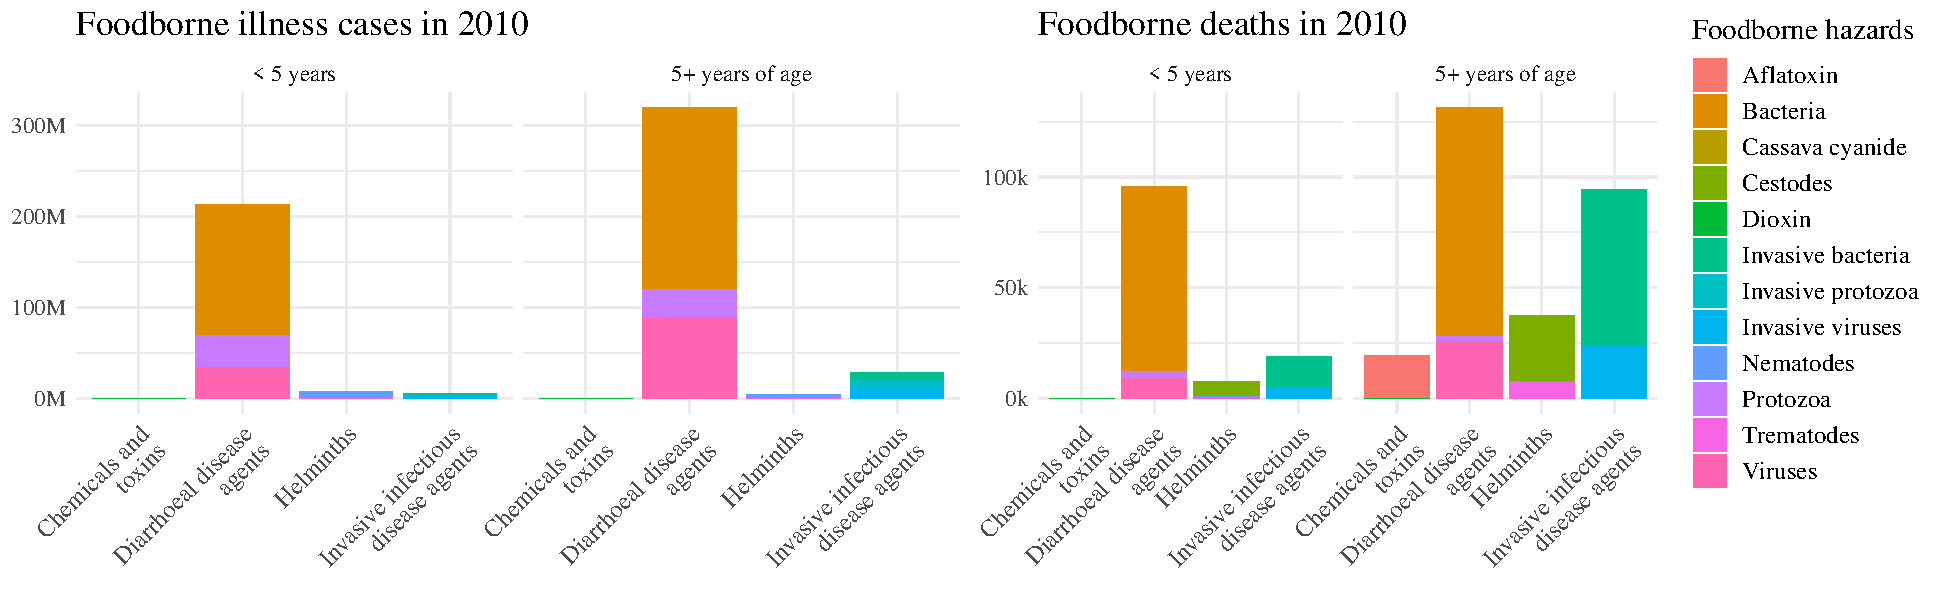
\includegraphics[width = \textwidth]{./Figures/chapter1/foodborneIllness/foodborneIllnessDeaths.pdf}
    \caption{Estimated number of foodborne illnesses and deaths in 2010 that were ascribed to different hazards, broken down into groups such as diarrhoeal disease agents, chemical and toxin hazards, helminths, and invasive infectious disease agents. Using hazard- and incidence-based methodologies, systematic reviews, surveillance data, and expert input, the WHO Foodborne Disease Burden Epidemiology Reference Group (FERG) produced the most recent estimates (2010). These plots offer a summary of the burden of foodborne illnesses worldwide. \citep{whoFoodborne2010Illnesses,whoFoodborne2010Deaths,whoBurden2015}}
    \label{fig:foodborneIllnesses}
\end{figure}

Most foodborne illnesses are caused by diarrhoeal disease agents, which include bacteria, protozoa, and viruses commonly found in farm animals and related products \citep{leeEtiological2021}. These pathogens affect the gut, producing toxins that disrupt proper water absorption and consequently cause diarrhoea; other symptoms may include fever, nausea, and abdominal cramps \citep{mathanDiarrhoeal1998, leeEtiological2021}. The most commonly known representatives  of this category include enterotoxigenic \textit{Escherichia coli} (ETEC) \citep{zhangEnterotoxigenic2022}, non-typhoidal \textit{Salmonella enterica} \citep{ferrariWorldwide2019} and Norovirus.

Invasive infectious disease agents are more aggressive, as they can enter the bloodstream, causing systemic issues like septicemia and meningitis \citep{hodgesInfectious2010}; indeed, these pathogens have a higher mortality rate than diarrhoeal agents \citep{kirkWorld2015}. Relevant examples of these pathogens include \textit{Listeria monocytogenes} \citep{camargoListeria2017}, \textit{Toxoplasma gondii}, and the virus of Hepatitis A \citep{dicolaFoodborne2021}.

Helminths, otherwise known as parasitic worms, are also worth mentioning when discussing foodborne illnesses, with \textit{Ascaris lumbricoides} \citep{leungHuman2021} and \textit{Taenia solium} \citep{ngwiliQualitative2021} being the most prominent members. Toxins and chemical agents also pose risks; they can be of biologicla origin, as in the case of aflatoxins from \textit{Aspergillus} fungi \citep{chaincontamRisk2020}, or they can be synthetic or man-made, like the dioxins that accumulate in fatty tissues of animals, which are later ingested by humans \citep{chaincontamRisk2018}. Moreover, inadequately processed foods like cassava can lead to cyanide poisoning \citep{okaforOccupational2002}, and bacterial byproducts like histamine in fish may cause scombroid poisoning \citep{landeteUpdated2008}. Finally, fertilizer and pesticide residues in food are able to affect health long-term if they are not properly removed \citep{kimExposure2017}.

\subparagraph{The multifaceted role of ammonium ion}
Ammonium ion (\amm{}) is a positively charged ion that derives from protonation of ammonia or that can be synthesized through hydrolysis of proteins and amino acids \citep{barracloughDirect1997}. Ammonium is a ubiquitous molecule that can be found in biological, environmental and food systems.
In food science, \amm{} plays a role in protein analysis, fermentation, and food safety. Indeed, it is produced during the process of protein decomposition, thus it can be correlated to protein content and food freshness \citep{wuEvaluation2022}. Moreover, \ce{NH4+} is a growth factor for yeasts and lactic acid bacteria in the production of wine and beer, where its levels must be strategically controlled to optimize the process and prevent formation of other dangerous compounds \citep{gomez-alonsoSimultaneous2007}. While \amm{}  itself is not directly toxic when ingested, excessive accumulation in the body, \eg{} in the presence of urea cycle disorders or liver damages, it can contribute to metabolic imbalances \cite{adevaAmmonium2012}.

\subparagraph{Histamine and food safety: understanding risks and prevention}

\begin{figure}[ht]
    \centering
    \subfloat[][Ammonium ion structure]{
        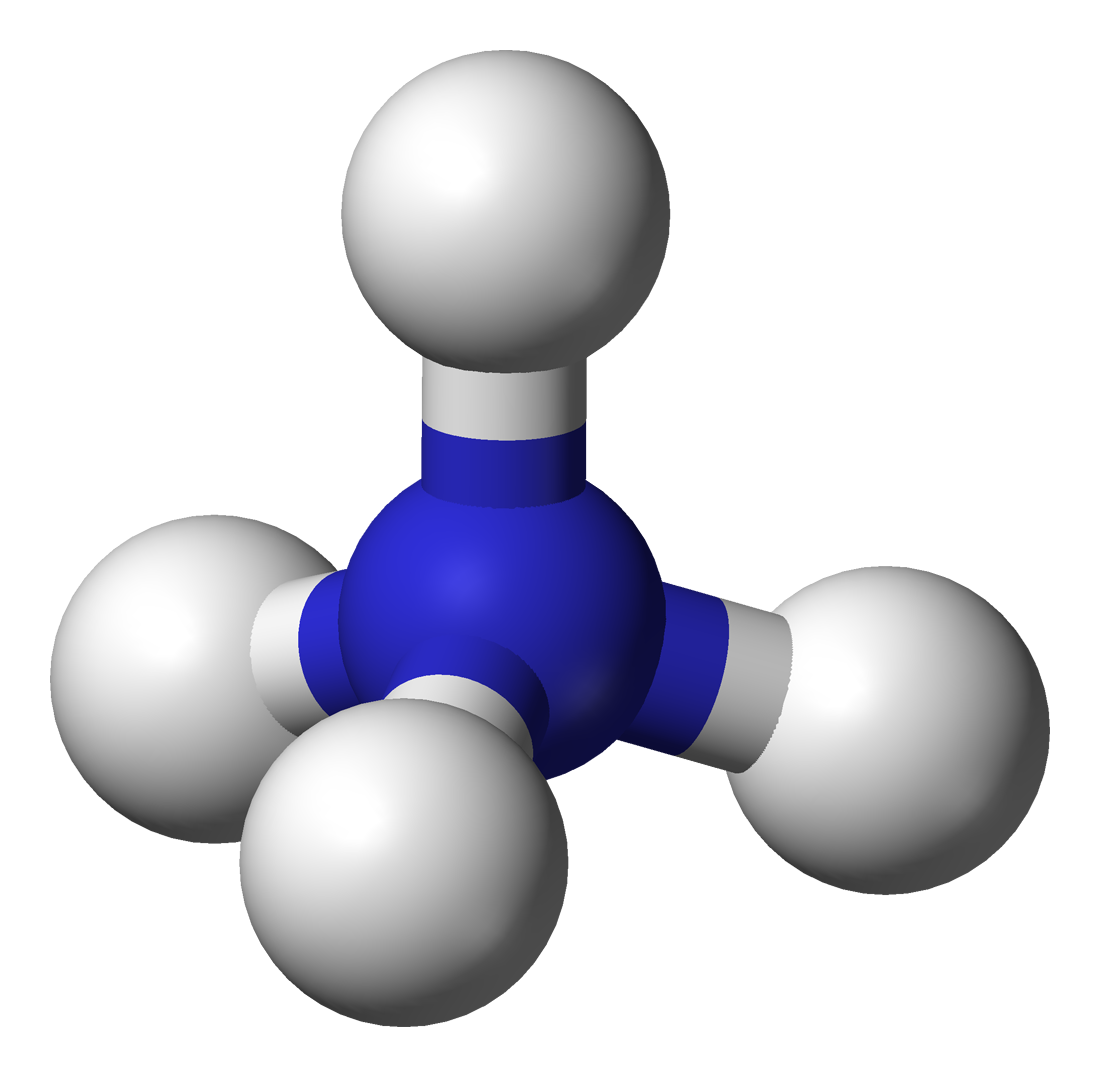
\includegraphics[width=0.25\textwidth]{figures/chapter1/foodborneIllness/ammonium.png}
    } \hspace{1cm}
    \subfloat[][Histamine structure]{
        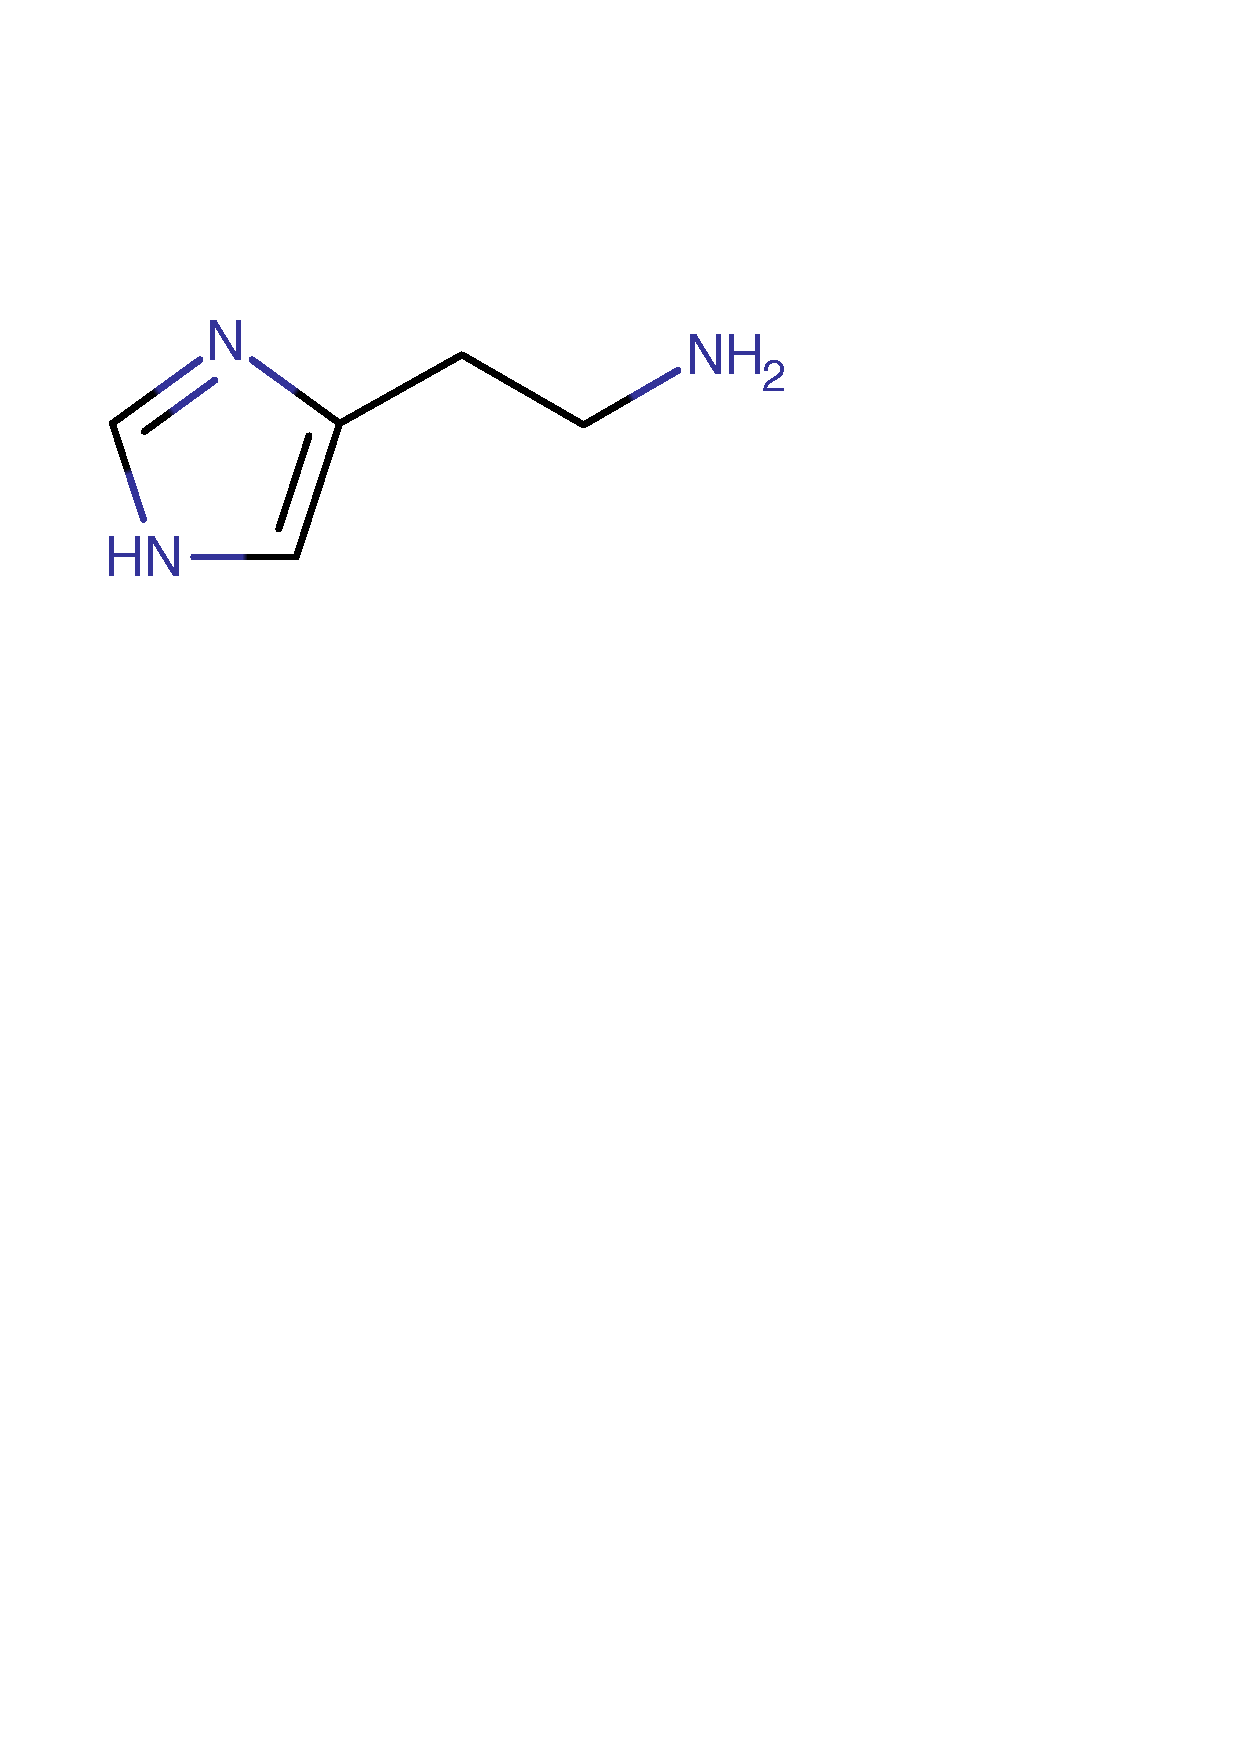
\includegraphics[width=0.4\textwidth]{figures/chapter1/foodborneIllness/histamine.pdf}
    }
    \caption{(a) Ammonium ion is the protonated form of ammonia, thus it is positively charged and it has the formula \amm{}.  Image source: Public Domain, Wikimedia Commons \citep{wikimediacommonsAmmonium2025}.
    (b) Histamine is a biogenic amine, \ie{} an organic compound containing nitrogen atoms. It consists of an imidazole ring linked to an ethylamine chain and it is synthesized in food through the decarboxylation of the amino acid histidine.}
    \label{fig:histamine}
\end{figure}

Histamine is a biogenic amine, \ie{} an organic compound that contains amine functional groups. Bacteria can synthesize it through many biochemical pathways, the most prevalent one being that of histidine decarboxylation \citep{maijalaEffect1993}; this process occurs in protein-rich foods such as scombroid fish (e.g., mackerel, tuna, sardines) \citep{halsteadFish1964} and fermented products \citep{spanoBiogenic2010, pretiFast2015}, especially when stored at improper temperatures, which increase bacterial growth and metabolism \citep{landeteUpdated2008}. The excessive consumption of histamine can result in a disease known as scombroid poisoning from the name of the fishes that cause it. This condition is characterized by some allergy-like symptoms such as rashes on the skin, localized redness and swelling, bronchoconstriction, and irritation of the eyes \citep{ozogulBiogenic2019, taylorHistamine1986}; chronic exposure may even cause it to be highly toxic and possibly carcinogenic through the formation of nitrosamines \citep{bartschRelevance1984}. Remarkably, since the discovery of scombroid poisoning, there has only been a single death reported that was linked to it \citep{taylorHistamine1989}. Despite the low mortality rate, rapid detection is essential for outbreak prevention; in fact, histamine is resistant to heat and cannot be degraded by cooking the food, indeed, it can even withstand treatment in an autoclave \citep{efsaScientific2015}. Thus, early detection and prevention become imperative for food safety. However, histamine detection presents some challenges: given that it is a metabolic byproduct rather than a live contaminant, its presence is difficult to attribute to a single bacterial species, so traditional detection methods (discussed in Section \ref{sec:traditional_detection}) may be inadequate and yield inconclusive results. Regulatory agencies have therefore set safety thresholds to minimize risk: the Food and Agriculture Organization/World Health Organization (FAO/WHO) defines a safe intake range of \SI{50}{mg} to \SI{200}{mg/kg} in a \SI{250}{g} serving of fish \citep{faowhoJoint2012}, while the United States Food and Drug Administration (US FDA) considers histamine dangerous at levels above \SI{500}{ppm}, thus enforcing a safety threshold of \SI{50}{ppm} \citep{fdaFish2022}. The European Food Safety Authority (EFSA) tolerates slightly higher limits, between \SIrange{100}{200}{ppm} \citep{strokaEquivalence2014}, still well below the toxic concentration.

\paragraph{Emergence and transmission of foodborne infections}
Foodborne illness can result from a variety of sources throughout the food chain. First of all, crop and animal infections may arise due to poor farming practices, such as using contaminated water and animal feed, and misusing pesticides and fertilizers \citep{whoBurden2015}. Secondly, poor hygiene practices during food handling increase contamination risks; these include inadequate handwashing by workers, cross-contamination between raw and ready-to-eat foods during preparation, and failure to maintain a safe temperature during storage and transportation \citep{toddFoodBorne2020}. Once a foodborne hazard is in food products, the interconnected nature of food supply chains amplifies its spread: indeed, increased international trade can cause pathogens to cross borders, turning isolated outbreaks into global health issues \citep{velusamyOverview2010}.

\paragraph{Foodborne illness prevention: a key strategy to avoid global outbreaks}
When a set of best practices is adopted at every level of the food chain, from the farming sector, to the food handling industries, down to the final consumers, foodborne illnesses can be drastically reduced or prevented.
These practices are encouraged and enforced by several regulatory organizations like WHO, EFSA, US FDA and more, by setting laws and promoting prevention and education campaigns for the public \citep{tauxeEmerging1997}.

In agriculture, good practices include using treated water for irrigation and animal care, along with maintaining proper sanitation throughout the entire process of growing, harvesting, and storing crops; these help in minimizing the risk of contamination at the source \citep{faoAssuring2003}.
A responsible use of antibiotics and pesticides is also fundamental to prevent foodborne illnesses. While antibiotics are effective in treating infections in both farming animals and plants, their overuse is rapidly contributing to the spread of antibiotics resistance, ultimately leaving farmers and people without adequate measures to counteract diseases \citep{canicaAntibiotic2019}. 
Pesticides, on the other hand, play a dual role in foodborne illness prevention. While some pesticides indeed reduce the growth of pathogens on plants, others may stimulate their proliferation \citep{dobhalSurvival2014}; it is also important to remember that the overuse of pesticides can itself lead to the occurrence of foodborne illnesses, as they are chemical contaminants associated with both short-term and chronic health effects. Overall, alternative preventative approaches, such as probiotics, plant-derived polyphenols, and bacteriophages, must be researched, to avoid antibiotics and pesticide use as precautionary measure \citep{friedmanAntibioticResistant2015,maAntimicrobial2019}.

For industries, food safety systems like Hazard Analysis and Critical Control Points (HACCP) have been implemented. These guidelines allow to identify potential risks and establish control measures to guarantee food safety during processing, storage, and distribution \citep{faowhoFAO2006,wallaceHACCP2014}. In addition, regular inspections, proper labeling, and traceability systems must be in place to ensure that contaminated goods can be quickly identified and removed from the market \citep{programFood2024,ISO2018}.

For individuals, the application of simple measures for maintaining proper hygiene during food preparation is essential; these include washing hands thoroughly, avoiding cross-contamination using different tools when working with different foods (\eg{} different knives and cutting boards for meat, fish, fruits and vegetables), and cooking foods to safe internal temperatures.
It is also important to preserve food at the proper temperature, \eg{} in the refrigerator or in the freezer and not consume it past its expiration date. If leftover remain after a meal, these should be left cooling down to room temperature to avoid raising the fridge internal temperature and favour bacterial growth. At the same time, food should be left at room temperature as little as possible, and when reheated, it should reach at least \SI{74}{\degreeCelsius} and not fall below \SI{57}{\degreeCelsius} \citep{whoFive2006,cdcFour2024,efsaHandling}. All together, these efforts can significantly reduce the risk of foodborne illnesses.

To prevent foodborne disease outbreaks, all levels and all sectors must cooperate with synergistic effort \citep{graceFood2017}. In this regard, governments and regulatory organizations bear a significant responsibility for establishing evidence-based regulations and consequently programming adequate interventions \citep{faoWorking2007}. Moreover, it is essential to invest towards the development of comprehensive national and supranational surveillance systems that can facilitate early detection of outbreaks before they result in adverse outcomes \citep{faoCodex2009}. Equally important are public awareness campaigns and training programs for individuals and for food producers and handlers, which help build a culture that prioritizes food safety at every level \citep{bosmanExpertise2016}.
